% Options for packages loaded elsewhere
\PassOptionsToPackage{unicode}{hyperref}
\PassOptionsToPackage{hyphens}{url}
%
\documentclass[
]{article}
\usepackage{amsmath,amssymb}
\usepackage{iftex}
\ifPDFTeX
  \usepackage[T1]{fontenc}
  \usepackage[utf8]{inputenc}
  \usepackage{textcomp} % provide euro and other symbols
\else % if luatex or xetex
  \usepackage{unicode-math} % this also loads fontspec
  \defaultfontfeatures{Scale=MatchLowercase}
  \defaultfontfeatures[\rmfamily]{Ligatures=TeX,Scale=1}
\fi
\usepackage{lmodern}
\ifPDFTeX\else
  % xetex/luatex font selection
\fi
% Use upquote if available, for straight quotes in verbatim environments
\IfFileExists{upquote.sty}{\usepackage{upquote}}{}
\IfFileExists{microtype.sty}{% use microtype if available
  \usepackage[]{microtype}
  \UseMicrotypeSet[protrusion]{basicmath} % disable protrusion for tt fonts
}{}
\makeatletter
\@ifundefined{KOMAClassName}{% if non-KOMA class
  \IfFileExists{parskip.sty}{%
    \usepackage{parskip}
  }{% else
    \setlength{\parindent}{0pt}
    \setlength{\parskip}{6pt plus 2pt minus 1pt}}
}{% if KOMA class
  \KOMAoptions{parskip=half}}
\makeatother
\usepackage{xcolor}
\usepackage[margin=1in]{geometry}
\usepackage{graphicx}
\makeatletter
\def\maxwidth{\ifdim\Gin@nat@width>\linewidth\linewidth\else\Gin@nat@width\fi}
\def\maxheight{\ifdim\Gin@nat@height>\textheight\textheight\else\Gin@nat@height\fi}
\makeatother
% Scale images if necessary, so that they will not overflow the page
% margins by default, and it is still possible to overwrite the defaults
% using explicit options in \includegraphics[width, height, ...]{}
\setkeys{Gin}{width=\maxwidth,height=\maxheight,keepaspectratio}
% Set default figure placement to htbp
\makeatletter
\def\fps@figure{htbp}
\makeatother
\setlength{\emergencystretch}{3em} % prevent overfull lines
\providecommand{\tightlist}{%
  \setlength{\itemsep}{0pt}\setlength{\parskip}{0pt}}
\setcounter{secnumdepth}{-\maxdimen} % remove section numbering
\ifLuaTeX
  \usepackage{selnolig}  % disable illegal ligatures
\fi
\usepackage{bookmark}
\IfFileExists{xurl.sty}{\usepackage{xurl}}{} % add URL line breaks if available
\urlstyle{same}
\hypersetup{
  pdftitle={Part B: Design Normalized Database},
  pdfauthor={Krishnappa, Kushal},
  hidelinks,
  pdfcreator={LaTeX via pandoc}}

\title{Part B: Design Normalized Database}
\author{Krishnappa, Kushal}
\date{Spring 2025}

\begin{document}
\maketitle

\subsection{\texorpdfstring{\textbf{1.
Introduction}}{1. Introduction}}\label{introduction}

This document presents a \textbf{normalized relational database schema}
for managing restaurant visits. The schema follows \textbf{Third Normal
Form (3NF)} to eliminate redundancy and ensure data integrity. The steps
involved include listing the initial \textbf{functional dependencies}
for a restaurant visit relation represented by all of the columns,
identifying \textbf{entities} and their relationships, performing
\textbf{decomposition} on identified \textbf{entities} and
\textbf{functional dependencies} to ensure normalization to 3NF, and
designing an \textbf{Entity-Relationship Diagram (ERD)} to illustrate
the final structure.

\subsection{\texorpdfstring{\textbf{2. Functional Dependencies
Identified For CSV
Data}}{2. Functional Dependencies Identified For CSV Data}}\label{functional-dependencies-identified-for-csv-data}

Initial data for the restaurant visits is a single relation represented
by all of the columns. The functional dependencies are identified from
the raw data to understand the relationships between the attributes.

\[
\text{VisitID} \rightarrow 
\left\{
\begin{array}{l}
\text{Restaurant}, \text{ServerEmpID}, \text{ServerName}, \text{StartDateHired}, \text{EndDateHired}, \text{HourlyRate}, \\
\text{ServerBirthDate}, \text{ServerTIN}, \text{VisitDate}, \text{VisitTime}, \text{MealType}, \text{PartySize}, \text{Genders}, \\
\text{WaitTime}, \text{CustomerName}, \text{CustomerPhone}, \text{CustomerEmail}, \text{LoyaltyMember}, \\
\text{FoodBill}, \text{TipAmount}, \text{DiscountApplied}, \text{PaymentMethod}, \text{OrderedAlcohol}, \text{AlcoholBill} 
\end{array}
\right\}
\]

\[
\text{ServerEmpID} \rightarrow 
\left\{
\begin{array}{l}
\text{ServerName}, \text{StartDateHired}, \text{EndDateHired}, \text{HourlyRate}, \text{ServerBirthDate}, \text{ServerTIN}
\end{array}
\right\}
\]

\[
\text{CustomerName} \rightarrow \{\text{CustomerPhone}, \text{CustomerEmail}, \text{LoyaltyMember}\}
\]

\subsection{\texorpdfstring{\textbf{3.
Normalization}}{3. Normalization}}\label{normalization}

\subsubsection{\texorpdfstring{\textbf{3.1 Entities Identified and
Attributes
Grouped}}{3.1 Entities Identified and Attributes Grouped}}\label{entities-identified-and-attributes-grouped}

\paragraph{\texorpdfstring{\textbf{1. Visit}}{1. Visit}}\label{visit}

\begin{itemize}
\tightlist
\item
  \textbf{key}: \texttt{VisitID}
\item
  \texttt{Restaurant}
\item
  \texttt{VisitDate}
\item
  \texttt{VisitTime}
\item
  \texttt{MealType}
\item
  \texttt{PartySize}
\item
  \texttt{Genders}
\item
  \texttt{WaitTime}
\end{itemize}

\paragraph{\texorpdfstring{\textbf{2. Server}}{2. Server}}\label{server}

\begin{itemize}
\tightlist
\item
  \textbf{key}: \texttt{ServerEmpID}
\item
  \texttt{ServerName}
\item
  \texttt{StartDateHired}
\item
  \texttt{EndDateHired}
\item
  \texttt{HourlyRate}
\item
  \texttt{ServerBirthDate}
\item
  \texttt{ServerTIN}
\end{itemize}

\paragraph{\texorpdfstring{\textbf{3.
Customer}}{3. Customer}}\label{customer}

\begin{itemize}
\tightlist
\item
  \textbf{key}: \texttt{CustomerID}
\item
  \texttt{CustomerPhone}
\item
  \texttt{CustomerName}
\item
  \texttt{CustomerEmail}
\item
  \texttt{LoyaltyMember}
\end{itemize}

\paragraph{\texorpdfstring{\textbf{4.
Billing}}{4. Billing}}\label{billing}

\begin{itemize}
\tightlist
\item
  \textbf{key}: \texttt{BillingID}
\item
  \texttt{FoodBill}
\item
  \texttt{TipAmount}
\item
  \texttt{DiscountApplied}
\item
  \texttt{PaymentMethod}
\item
  \texttt{orderedAlcohol}
\item
  \texttt{AlcoholBill}
\end{itemize}

\paragraph{\texorpdfstring{\textbf{Relationship Between Identified
Entities}}{Relationship Between Identified Entities}}\label{relationship-between-identified-entities}

\paragraph{1. Visit - Customer Relationship
(One-to-Many)}\label{visit---customer-relationship-one-to-many}

\begin{itemize}
\tightlist
\item
  \textbf{Explanation}: A \textbf{customer} can make multiple
  \textbf{visits}, but each \textbf{visit} is associated with a single
  \textbf{customer}.
\item
  \textbf{Cardinality}: \textbf{1 Customer → M Visits} (1:N)
\end{itemize}

\paragraph{2. Visit - Server Relationship
(One-to-Many)}\label{visit---server-relationship-one-to-many}

\begin{itemize}
\tightlist
\item
  \textbf{Explanation}: A \textbf{server} can attend multiple
  \textbf{visits}, but each \textbf{visit} is handled by a single
  \textbf{server}.
\item
  \textbf{Cardinality}: \textbf{1 Server → M Visits} (1:N)
\end{itemize}

\paragraph{3. Visit - Billing Relationship
(One-to-One)}\label{visit---billing-relationship-one-to-one}

\begin{itemize}
\tightlist
\item
  \textbf{Explanation}: Each \textbf{visit} has exactly \textbf{one}
  related \textbf{billing entry}, and each \textbf{billing entry}
  belongs to exactly \textbf{one visit}.
\item
  \textbf{Cardinality}: \textbf{1 Visit → 1 Billing} (1:1)
\end{itemize}

\subsubsection{\texorpdfstring{\textbf{3.2 Approach To
Normalization}}{3.2 Approach To Normalization}}\label{approach-to-normalization}

\begin{itemize}
\item
  \textbf{1NF}: Each attribute is atomic. All the tables have separate
  columns for ID's which will uniquely identify each row.
\item
  \textbf{2NF}: Partial dependencies are eliminated by decomposing the
  relation into multiple relations and ensuring each relation has a
  single primary key.
\item
  \textbf{3NF}: Transitive dependencies are removed by creating separate
  relations for the dependent attributes.
\end{itemize}

\textbf{Functional Dependencies From Normalized Database}

\[
\text{PaymentID} \rightarrow \{\text{PaymentMethod}\}
\]

\[
\text{CustomerID} \rightarrow \{\text{CustomerName}, \text{CustomerPhone}, \text{CustomerEmail}, \text{LoyaltyMember}\}
\]

\[
\text{RestaurantID} \rightarrow \{\text{RestaurantName}\}
\]

\[
\text{MealTypeID} \rightarrow \{\text{MealType}\}
\]

\[
\text{ServerEmpID} \rightarrow 
\left\{
\begin{array}{l}
\text{ServerName}, \text{StartDateHired}, \text{EndDateHired}, \text{HourlyRate}, \text{ServerBirthDate}, \text{ServerTIN}
\end{array}
\right\}
\]

\[
\text{VisitID} \rightarrow 
\left\{
\begin{array}{l}
\text{RestaurantID}, \text{ServerEmpID}, \text{VisitDate}, \text{VisitTime}, \text{MealTypeID}, \text{PartySize}, \text{Genders}, \\
\text{WaitTime}, \text{CustomerID}
\end{array}
\right\}
\]

\[
\text{BillID} \rightarrow 
\left\{
\begin{array}{l}
\text{VisitID}, \text{FoodBill}, \text{TipAmount}, \text{DiscountApplied}, \text{PaymentID}, \text{OrderedAlcohol}, \\
\text{AlcoholBill}
\end{array}
\right\}
\]

\subsection{\texorpdfstring{\textbf{4. ERD for Normalized
Tables}}{4. ERD for Normalized Tables}}\label{erd-for-normalized-tables}

\textbf{Entity-Relationship Diagram (ERD) in Crow's Foot Notation}

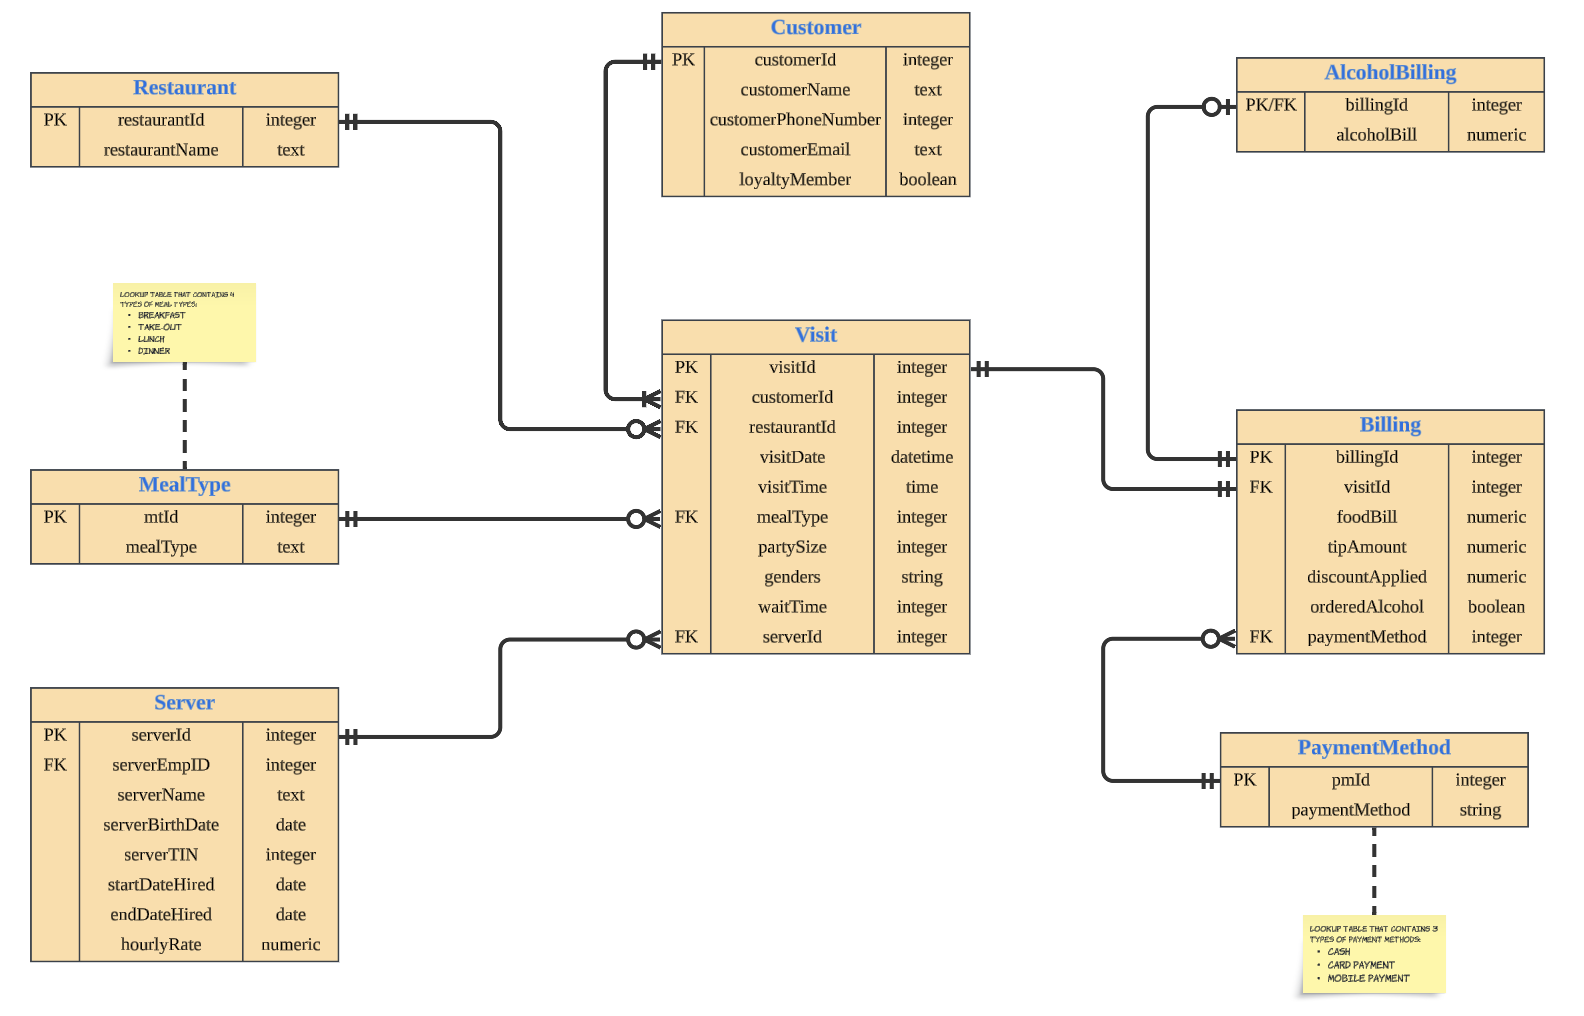
\includegraphics{ERD.png}

\end{document}
